\chapter{Implementation} \label{ch:implementation}

\section{Design and Architecture}
The design of the implementation leverages a microservices architecture to simulate real-world data collection and processing. The system was designed to emulate a sensor-driven environment, utilizing containerized services for data generation, communication, transformation, and visualization.

To simulate real sensors or microcontrollers, a python application was developed. This application processes a real dataset of air quality data and extracts the data corresponding to specific timestamps. The extracted data is then published to an MQTT broker. This python application is packaged in a Docker image to enable scalability and reusability. Multiple instances of this sensor simulation image are deployed as separate Docker containers, each simulating an independent sensor.

To enable communication using the MQTT protocol between the simulated sensors and the data-processing layer, an MQTT broker was deployed. The MQTT broker, also packaged in a Docker container, receives data from the sensor containers and forwards it to the subscribed clients.

A controller service was implemented as a Python application. This application subscribes to the MQTT topics published by the sensors, processes the incoming data, and converts it into a format compatible with Prometheus. The transformed data is then exposed through an HTTP endpoint. The controller application is also containerized and deployed as a separate Docker container.

Prometheus was deployed in a Docker container and configured to periodically scrape the data exposed by the controller service and to retain it for an appropriate amount of time.

Finally, Grafana was deployed as the visualization layer of the system, again in its own Docker container. Grafana was configured to use Prometheus as its data source. Custom dashboards were created to visualize the air quality data collected from the simulated sensors, enabling real-time monitoring and analysis.

The entire system was deployed using Docker Compose to allow for a easy orchestration and management of all the containerized services and for a straightforward, scalable and reproducible deployment.

\begin{figure}[!h]
    \graphicspath{ {./diagrams/} }
    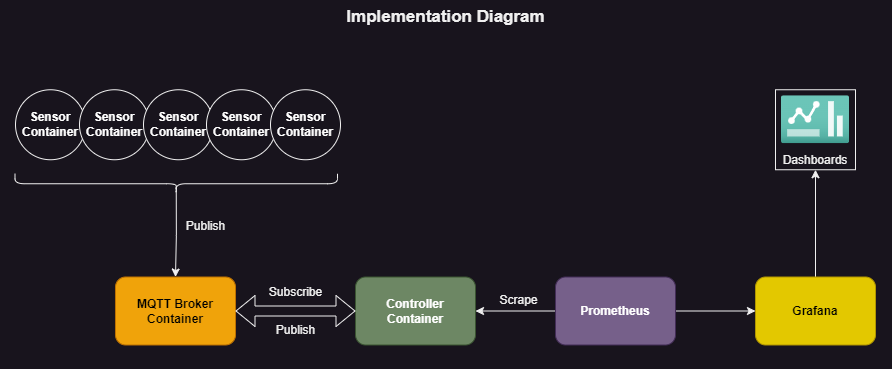
\includegraphics[scale=0.55]{implementation.png}
    \centering
    \caption{Implementation Diagram}
    \label{fig:imple_dia}
\end{figure}

\section{Dataset}
\subsection{Dataset Description}
The dataset used contains the responses of a gas multisensor device deployes on the field in an Italian city. Hourly responses averages are recorded along with gas concentrations references from a certified analyzer. The dataset contains 9357 instances of hourly averaged responses from an array of 5 metal oxide chemical sensors embedded in an Air Quality Chemical Multisensor Device. Ground Truth hourly averaged concentrations for CO, Non Metanic Hydrocarbons, Benzene, Total Nitrogen Oxides (NOx) and Nitrogen Dioxide (NO2) were provided by a co-located reference certified analyzer. Dataset can be found \href{https://www.kaggle.com/datasets/fedesoriano/air-quality-data-set/data}{here}.

\begin{table}[!h]
\begin{tabular}{|c|p{0.8\linewidth}|}
    \hline
    \multicolumn{2}{|c|}{\textbf{Attribute Information}} \\
    \hline
    \hline
    0& Date (DD/MM/YYYY) \\ \hline
    1& Time (HH.MM.SS) \\ \hline
    2& True hourly averaged concentration CO in $mg/m^3$ (reference analyzer) \\ \hline
    3& PT08.S1 (tin oxide) hourly averaged sensor response (nominally CO targeted) \\ \hline
    4& True hourly averaged overall Non Metanic HydroCarbons concentration in $microg/m^3$ (reference analyzer) \\ \hline
    5& True hourly averaged Benzene concentration in $microg/m^3$ (reference analyzer) \\ \hline
    6& PT08.S2 (titania) hourly averaged sensor response (nominally NMHC targeted) \\ \hline
    7& True hourly averaged NOx concentration in ppb (reference analyzer) \\ \hline
    8& PT08.S3 (tungsten oxide) hourly averaged sensor response (nominally NOx targeted) \\ \hline
    9& True hourly averaged NO2 concentration in $microg/m^3$ (reference analyzer) \\ \hline
    10& PT08.S4 (tungsten oxide) hourly averaged sensor response (nominally NO2 targeted) \\ \hline
    11& PT08.S5 (indium oxide) hourly averaged sensor response (nominally O3 targeted) \\ \hline
    12& Temperature in °C \\ \hline
    13& Relative Humidity (\%) \\ \hline
    14& AH Absolute Humidity  \\ \hline
\end{tabular}
\centering
\caption{Dataset Attribute Information}
\label{fig:dataset_attri}
\end{table}

\subsection{Dataset Manipulation}
Dataset was originally formatted in comma-separated values (CSV) format to be easily imported in a spreadsheet. To bring the CSV formatted dataset in a programmatically friendlier json format, a python script was developed. 
To assist with the randomized nature of data generation by the sensor simulator, for every timestamp a json object was created, with key an incremental integer and value the collection of metrics in json object format. Also empty rows were removed.

\begin{minted}[%
    framesep=2mm,
    baselinestretch=1.2,
    bgcolor=LightGray,
    fontsize=\footnotesize,
    breaklines
    ]{python}
    import csv
    import sys
    import json
    import os

    # Creates a new csv file named 'edited_csv' that doesn't contain empty rows, or rows with empty fields
    def csv_cleanup(csvfilename):
        with open(csvfilename, newline='') as csvfile:
            with open('edited_csv', 'w', newline='') as edited_csvfile:
                original = csv.reader(csvfile, delimiter=';')
                edited = csv.writer(edited_csvfile, delimiter=';')
                # fieldnames = next(original)
                # fieldnames.insert(0, "#")
                # edited.writerow(fieldnames)
                # i = 1
                for row in original:
                    if row and any(row) and any(field.strip() for field in row):
                        # row.insert(0, i)
                        edited.writerow(row)
                        # i += 1

    # Creates a json file from the edited csv file with an incremental integer as keys
    def csv_to_json(filename):
        data_dict = {}
        with open('edited_csv', newline='') as csvfile:
            edited = csv.DictReader(csvfile, delimiter=';')
            key = 1
            for row in edited: 
                data_dict[key] = row
                key += 1
        with open(filename+'.json', 'w') as jsonfile:
            jsonfile.write(json.dumps(data_dict, indent = 4))



    csvfilename = sys.argv[1]
    filename = csvfilename.split('/')[-1].split('.')[0]

    csv_cleanup(csvfilename)
    csv_to_json(filename)
    os.remove('edited_csv')
\end{minted}

The json re-formated dataset is structured as seen below.

\begin{minted}[%
    framesep=2mm,
    baselinestretch=1.2,
    bgcolor=LightGray,
    fontsize=\footnotesize,
    breaklines
    ]{json}
    {
        "1": {
            "Date": "10/03/2004",
            "Time": "18.00.00",
            "CO(GT)": "2,6",
            "PT08.S1(CO)": "1360",
            "NMHC(GT)": "150",
            "C6H6(GT)": "11,9",
            "PT08.S2(NMHC)": "1046",
            "NOx(GT)": "166",
            "PT08.S3(NOx)": "1056",
            "NO2(GT)": "113",
            "PT08.S4(NO2)": "1692",
            "PT08.S5(O3)": "1268",
            "T": "13,6",
            "RH": "48,9",
            "AH": "0,7578",
            "": ""
        },
        "2": {
            "Date": "10/03/2004",
            "Time": "19.00.00",
            "CO(GT)": "2",
            "PT08.S1(CO)": "1292",
            "NMHC(GT)": "112",
            "C6H6(GT)": "9,4",
            "PT08.S2(NMHC)": "955",
            "NOx(GT)": "103",
            "PT08.S3(NOx)": "1174",
            "NO2(GT)": "92",
            "PT08.S4(NO2)": "1559",
            "PT08.S5(O3)": "972",
            "T": "13,3",
            "RH": "47,7",
            "AH": "0,7255",
            "": ""
        }
    }
\end{minted}

\section{Sensor Simulator}
\subsection{Scenario}
The sensors remain in a low-power idle state to conserve energy. They are subscribed to the "collect-data" topic but are not actively collecting or publishing data. The controller node publishes a message to the MQTT topic "collect-data". This message is broadcast to all subscribed sensors by the MQTT broker. Upon receiving the trigger from the collect-data topic, sensors begin collecting air quality metrics. After collecting the data, each sensor publishes its metrics to its respective MQTT topic and returns to an idle state.
\subsection{Application}
As described on the scenario, first action on the application is establishing a connection to the MQTT broker, making sure to reconnect in case of disconnection, which would happen often in a real case scenario utilizing an unreliable cellular connection and subscribing to the "collect-data" topic. Then, once a message from the topic is received the data collection and publishing script is executed.

\begin{minted}[%
    framesep=2mm,
    baselinestretch=1.2,
    bgcolor=LightGray,
    fontsize=\footnotesize,
    breaklines
    ]{python}
    import socket
    import time
    import subprocess
    import paho.mqtt.client as mqtt_client

    port = 1883  # Default port for MQTT communication
    topic = "collect-data"  # Topic to subscribe to for data collection
    hostname = socket.gethostname()  # Get the hostname of the machine running this script. Machine (container) hostname is enforced later-on by docker compose 
    client_id = 'subscribe-{}'.format(hostname)  # Unique client ID for MQTT connection
    # broker = 'localhost'  # Uncomment this line for local broker testing
    broker = 'host.docker.internal'  # Use when running in a Docker environment

    def connect_mqtt():
        """
        Connects to the MQTT broker and sets up event handlers for connect, disconnect, and message events.
        """

        def on_connect(client, userdata, flags, rc):
            """
            Callback triggered upon connecting to the MQTT broker.
            """
            if rc == 0:
                print("Connected to MQTT Broker!")
                client.subscribe(topic)  # Subscribe to the specified topic
            else:
                print("Failed to connect, return code %d\n", rc)
        
        def on_disconnect(client, userdata, rc):
            """
            Callback triggered when the MQTT client disconnects from the broker.
            Implements an exponential backoff strategy for reconnection attempts.
            """
            FIRST_RECONNECT_DELAY = 1
            RECONNECT_RATE = 2
            MAX_RECONNECT_COUNT = 12
            MAX_RECONNECT_DELAY = 60

            print("Disconnected with result code: %s", rc)
            reconnect_count, reconnect_delay = 0, FIRST_RECONNECT_DELAY
            while reconnect_count < MAX_RECONNECT_COUNT:
                print("Reconnecting in {} seconds...".format(reconnect_delay))
                time.sleep(reconnect_delay)

                try:
                    client.reconnect()
                    print("Reconnected successfully!")
                    return
                except Exception as err:
                    print("{}. Reconnect failed. Retrying...".format(err))

                reconnect_delay *= RECONNECT_RATE
                reconnect_delay = min(reconnect_delay, MAX_RECONNECT_DELAY)
                reconnect_count += 1
            print("Reconnect failed after {} attempts. Exiting...".format(reconnect_count))

        def on_message(client, userdata, msg):
            """
            Callback triggered when a message is received on the subscribed topic.
            """
            print("Received `{}` from `{}` topic".format(msg.payload.decode(), msg.topic))
            subprocess.run(["./sensor_data"])  # Execute the sensor_data script upon message receipt

        # Create an MQTT client instance, assign the callback functions and connect
        client = mqtt_client.Client(client_id)
        client.on_connect = on_connect
        client.on_disconnect = on_disconnect
        client.on_message = on_message
        client.connect(broker, port)
        return client  # Return the configured client instance

    def run():
        """
        Main function to connect the MQTT client and start its loop.
        """
        client = connect_mqtt()
        client.loop_forever()

    if __name__ == '__main__':
        run()
\end{minted}

The data collection script, again starts by establishing a connection client with the MQTT broker. Once connection is established, the data collection process starts. To simulate a real-world scenario, to add variation between the multiple sensors and a randomization element, that also prolongs the use of the dataset before going over the same data, an elaborate process was devised. To ensure the randomized data have a real-world, logical flow, the next data point is selected from the range (previous - 2, previous + 3). This ensures that the metrics collected each time are only a few hours apart instead of completely random, which would result in completely abnormal differences on metrics that wouldn't be observed on metrics taken a few minutes or an hour apart. It also ensures that the data point slowly moves forward in time, as to not overly repeat the same data. The starting point for this process is randomized using another script, to ensure results between sensors don't overlap heavily. Since the data collection process is ephemeral, the data points needs to be stored. This could have been achieved in a number of ways, like passing it back and forth between the main subscription script or using an environmental variable, but storing to a file was preferred as it could also be utilized if a recovery scenario was to be covered. Once the end of the database is reached, a new starting point is, again, randomly selected.

\begin{minted}[%
    framesep=2mm,
    baselinestretch=1.2,
    bgcolor=LightGray,
    fontsize=\footnotesize,
    breaklines
    ]{python}
    import json
    import random, os
    import socket
    import subprocess
    from dotenv import load_dotenv
    import paho.mqtt.client as mqtt_client

    port = 1883  # Default port for MQTT communication
    hostname = socket.gethostname()  # Retrieve the hostname of the current machine. Hostname is enforced by docker compose.
    topic = "sensor-data/{}".format(hostname)  # Define the unique topic for publishing sensor data
    client_id = 'publish-{}'.format(hostname)  # Unique client ID for MQTT connection
    # broker = 'localhost'  # Uncomment this line for local broker testing
    broker = 'host.docker.internal'  # Use this broker when running in a Docker environment

    def connect_mqtt():
        """
        Connects to the MQTT broker and sets up the on_connect callback.
        """

        def on_connect(client, userdata, flags, rc):
            """
            Callback triggered upon connecting to the MQTT broker.
            """
            if rc == 0:
                print("Connected to MQTT Broker!")
            else: 
                print("Failed to connect, return code %d\n", rc)

        client = mqtt_client.Client(client_id)
        client.on_connect = on_connect 
        client.connect(broker, port)  
        return client  

    def data_gen():
        """
        Generates sensor data by selecting a random entry from a dataset.
        The selection point is controlled via an environment variable.
        """
        with open("dataset.json") as datafile:
            json_data = json.load(datafile)  # Load the dataset from the JSON file
        
            load_dotenv()  # Load environment variables from the .env file
            startpoint = int(os.getenv('STARTPOINT'))  # Get the STARTPOINT from the .env file
            # Randomize the data selection around the startpoint. Slowly moves forward in time, while keeping results semi-random and ensuring a logical history.
            randomizer = random.randint(startpoint - 2, startpoint + 3)
            while randomizer not in range(1, len(json_data)):  # Ensure the randomizer is valid
                subprocess.run(["./set_startpoint"])  # Run a script to reset the startpoint
                load_dotenv()  # Reload environment variables
                startpoint = int(os.getenv('STARTPOINT'))
                randomizer = random.randint(startpoint - 10, startpoint + 10)

            # Update the STARTPOINT in the .env file
            with open(".env", "w") as f:
                f.write("STARTPOINT={}".format(randomizer))

            randata = json_data[str(randomizer)]  # Fetch the random data entry
            return randata  # Return the selected data

    def publish(client, data):
        """
        Publishes a message to the MQTT topic.
        """
        msg = str(data)  # Convert the data to a string
        result = client.publish(topic, msg)  # Publish the message to the topic
        status = result[0]  # Check the result status
        if status == 0:
            print("Sent `{}` to topic `{}`".format(msg, topic))
        else:
            print("Failed to send message to topic {}".format(topic))        

    if __name__ == '__main__':
        client = connect_mqtt()  # Establish the MQTT connection
        client.loop_start()  # Start the MQTT client loop in a separate thread
        randata = data_gen()  # Generate random sensor data
        publish(client, randata)  # Publish the generated data to the topic
        client.loop_stop()  # Stop the MQTT client loop
\end{minted}

\begin{minted}[%
    framesep=2mm,
    baselinestretch=1.2,
    bgcolor=LightGray,
    fontsize=\footnotesize,
    breaklines
    ]{python}
    import json, random

    def set_startpoint():
        """
        Sets a STARTPOINT value based on the dataset's size and writes it to an .env file.
        """
        with open("dataset.json") as datafile:
            json_data = json.load(datafile) # Load the dataset from a JSON file
            
            endpoint = round(len(json_data)/10) # Determine the upper limit for the STARTPOINT range
            startpoint = str(random.randint(1, endpoint))

            print("Setting STARTPOINT as {}".format(startpoint))

            with open(".env", "w") as f:
                f.write("STARTPOINT={}".format(startpoint)) # Write the STARTPOINT to the .env file

    if __name__ == '__main__':
        set_startpoint()
\end{minted}

Only libraries required, are "paho-mqtt" and "python-dotenv".

\subsection{Containerization}
IoT sensors usually are embedded on microcontrollers with limited hardware resources. While minimal, optimized subsets of Python do exist, building the Python scripts and using the binaries directly, makes more sense. To stick with the minimal, lightweight enviroment expected in an IoT microcontroller, a minimal linux docker image as base is a good fit. The \href{https://hub.docker.com/_/alpine/}{Alpine docker image} was selected, as it is the industry standard for minimal, striped down Linux images, and current latest ones are only around 5MB uncompressed. To build the Python scripts PyInstaller was used, but because Alpine utilizes \href{https://musl.libc.org/}{Musl C library}, instead of the \href{https://www.gnu.org/software/libc/}{GNU C library}, a third party PyInstaller-ready, Alpine-based Python image was used, that can be found \href{https://github.com/six8/pyinstaller-alpine}{here}. Using this image also removes the requirement of installing PyInstaller, a great example of how docker removes environmental dependencies. The following command was used:
\begin{minted}[%
    framesep=2mm,
    baselinestretch=1.2,
    bgcolor=LightGray,
    fontsize=\footnotesize,
    breaklines
    ]{bash}
    $ docker run --rm -v "${PWD}:/src" anastzampetis/pyinstaller-alpine --noconfirm --onefile --log-level DEBUG --clean <script_name>.py
\end{minted}
Once the binaries were built, a simple Dockerfile was used to copy the binaries and the json formated dataset into the base Alpine image and set the binaries to be executed when running the container.
\begin{minted}[%
    framesep=2mm,
    baselinestretch=1.2,
    bgcolor=LightGray,
    fontsize=\footnotesize,
    breaklines
    ]{dockerfile}
    FROM alpine

    WORKDIR /app
    ADD dist/sensor_data .
    ADD dist/sensor_sub .
    ADD dist/set_startpoint .
    ADD dataset.json .

    CMD ./set_startpoint && ./sensor_sub
\end{minted}  
Finally to build the image, below command was executed:
\begin{minted}[%
    framesep=2mm,
    baselinestretch=1.2,
    bgcolor=LightGray,
    fontsize=\footnotesize,
    breaklines
    ]{bash}
    $ docker build -t anastzampetis/sensor-emul:latest -f Dockerfile .
\end{minted}

\section{MQTT Broker}
For the MQTT broker, the Eclipse Mosquitto MQTT broker was selected. Mosquitto is an open-source message broker that implements the MQTT protocol. Mosquitto is designed to be small and efficient, suitable for IoT devices with constrained resources, and fits well in a microservice enviroment. It's also very capable of handling even large-scale deployments, making it a good fit for a scalable enviroment.

To stay true to a microservice architecture and to make deployment and management easier, the Mosquitto MQTT broker was deployed in a docker container. It is already available in an official image found \href{https://hub.docker.com/_/eclipse-mosquitto}{here}. Configuring the container was simple in the scope of this implementation, since there was no need for secutiry protocols and persisting data inside the broker container because Prometheus is utilized.

\begin{minted}[%
    framesep=2mm,
    baselinestretch=1.2,
    bgcolor=LightGray,
    fontsize=\footnotesize,
    breaklines
    ]{bash}
    persistence false     # No need to persist data, since it's pushed to Prometheus
    listener 1883         # The listener port that clients publish to
    allow_anonymous true  # Since there is no need for security, anonymous is allowed.
\end{minted}

\section{Controller Node}
The controller node serves a number of important functions. Firstly, it's responsible for publishing on the "collect-data" MQTT topic, so the sensor simulators will leave the idle state and collect the data. Then, by subscribing to the topics the sensors publish to, "sensor-data/\#" (usign a wildcard topic definition also allows for scaling of sensors), the controller node will receive messages from each topic, containing the sensor data.

Once these messages are received, using the "prometheus\_client" library all metrics are converted in Prometheus format and exposed to an endpoint. Every metric is assigned to a different Gauge type Prometheus metric and labeled usign the sensor unique id. A gauge is a metric that represents a single numerical value that can arbitrarily go up and down. This part of the controller's functionality is essensially a Prometheus exporter.

Usually Prometheus exporters collect data periodically, but continiously expose last collected metrics on an HTTP endpoint. In this case, thought, to make it easier to change the rate of data collection, by changing the scraping rate of Prometheus, a different design was implemented. The controller, utilizing the "fastapi" library and "gunicorn" exposes an API endpoint. When Prometheus scrapes this endpoint, the data collection process is triggered by the controller, and after a small time delay the controller respondes with the metrics. 

<add scripts>
<add output of controller>
<add captions on the code?>

\section{Prometheus}

\section{Grafana}

\section{Orchestration}
